\documentclass{article}
 
\usepackage{fullpage}
\usepackage{color}
\usepackage{amsmath}
\usepackage{url}
\usepackage{verbatim}
\usepackage{graphicx}
\usepackage{parskip}
\usepackage{amssymb}
\usepackage{nicefrac}
\usepackage{listings} % For displaying code
\usepackage{algorithm2e} % pseudo-code

% Answers
\def\ans#1{\par\gre{Answer: #1}}
%\def\ans#1{} % Comment this line to produce document with answers

% Colors
\definecolor{blu}{rgb}{0,0,1}
\def\blu#1{{\color{blu}#1}}
\definecolor{gre}{rgb}{0,.5,0}
\def\gre#1{{\color{gre}#1}}
\definecolor{red}{rgb}{1,0,0}
\def\red#1{{\color{red}#1}}
\def\norm#1{\|#1\|}

% Math
\def\R{\mathbb{R}}
\def\argmax{\mathop{\rm arg\,max}}
\def\argmin{\mathop{\rm arg\,min}}
\newcommand{\mat}[1]{\begin{bmatrix}#1\end{bmatrix}}
\newcommand{\alignStar}[1]{\begin{align*}#1\end{align*}}
\def\half{\frac 1 2}
\def\cond{\; | \;}


% LaTeX
\newcommand{\fig}[2]{\includegraphics[width=#1\textwidth]{a4f/#2}}
\newcommand{\centerfig}[2]{\begin{center}\includegraphics[width=#1\textwidth]{a4f/#2}\end{center}}
\newcommand{\matCode}[1]{\lstinputlisting[language=Matlab]{a4f/#1.m}}
\def\items#1{\begin{itemize}#1\end{itemize}}
\def\enum#1{\begin{enumerate}#1\end{enumerate}}


\begin{document}

\title{CPSC 340 Assignment 4  (due Friday November 1 at 11:55pm)}
\author{}
\date{}
\maketitle
\vspace{-4em}



\section{Gaussian RBFs and Regularization}

Unfortunately, in practice we often don't know what basis to use. However, if we have enough data then we can make up for this by using a basis that is flexible enough to model any reasonable function. These may perform poorly if we don't have much data, but can perform almost as well as the optimal basis as the size of the dataset grows. In this question you will explore using Gaussian radial basis functions (RBFs), which have this property. These RBFs depend on a parameter $\sigma$, which (like $p$ in the polynomial basis) can be chosen using a validation set. In this question, you will also see how cross-validation allows you to tune parameters of the model on a larger dataset than a strict training/validation split would allow.

\subsection{Regularization}

If you run the demo \emph{example\_RBF.jl}, it will load a dataset and randomly split the training examples into a ``train" and a ``validation" set (it does this randomly since the data is sorted). It will then search for the best value of $\sigma$ for the RBF basis. Once it has the ``best" value of $\sigma$, it re-trains on the entire dataset and reports the training error on the full training set as well as the error on the test set.

A strange behaviour appears: if you run the script more than once it might choose different values of $\sigma$. Sometimes it chooses a large value of $\sigma$ (like $32$) that follows the general trend but misses the oscillations. Other times it sets $\sigma = 1$ or $\sigma=2$, which fits the oscillations better but overfits so achieves a similar test error.\footnote{This behaviour seems to be dependent on your exact setup. Because the $Z^TZ$ matrix with the RBF matrix is really-badly behaved numerically, different floating-point and matrix-operation implementations will handle this in different ways: in some settings it will actually regularizer for you!} \blu{Modify the \emph{leastSquaresRBF} function so that it allows a regularization parameter $\lambda$ and it fits the model with L2-regularization. Hand in your code, and report and describe how the performance changes if you use a regularized estimate with $\lambda = 10^{-12}$ (a very small value).}
Hint: to construct an identity matrix in Julia, use the linear algebra package (\emph{using LinearAlgebra}) and then use $I$ to make an identity matrix of the appropriate size (Julia figures out the dimensions for you).
\ans{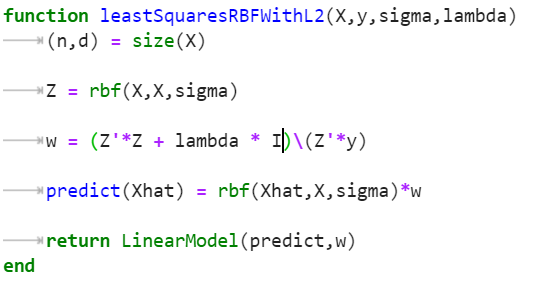
\includegraphics[width=10cm]{Q1.PNG} \\
Running the script multiple times, the optimal $\sigma$ will be less likely to change from 1.}


\subsection{Cross-Validation}

Even with regularization, the randomization of the training/validation sets has an effect on the value of $\sigma$ that we choose (on some runs it still chooses a large $\sigma$ value).
This variability would be reduced if we had a larger ``train" and ``validation" set, and one way to simulate this is with \emph{cross-validation}. \blu{Modify the training/validation procedure to use 10-fold cross-validation to select $\sigma$, and hand in your code. How does this change the performance when fixing $\lambda = 10^{-12}$?}\footnote{In practice, we typically use cross-validation to choose both $\sigma$ and $\lambda$}
\ans{ 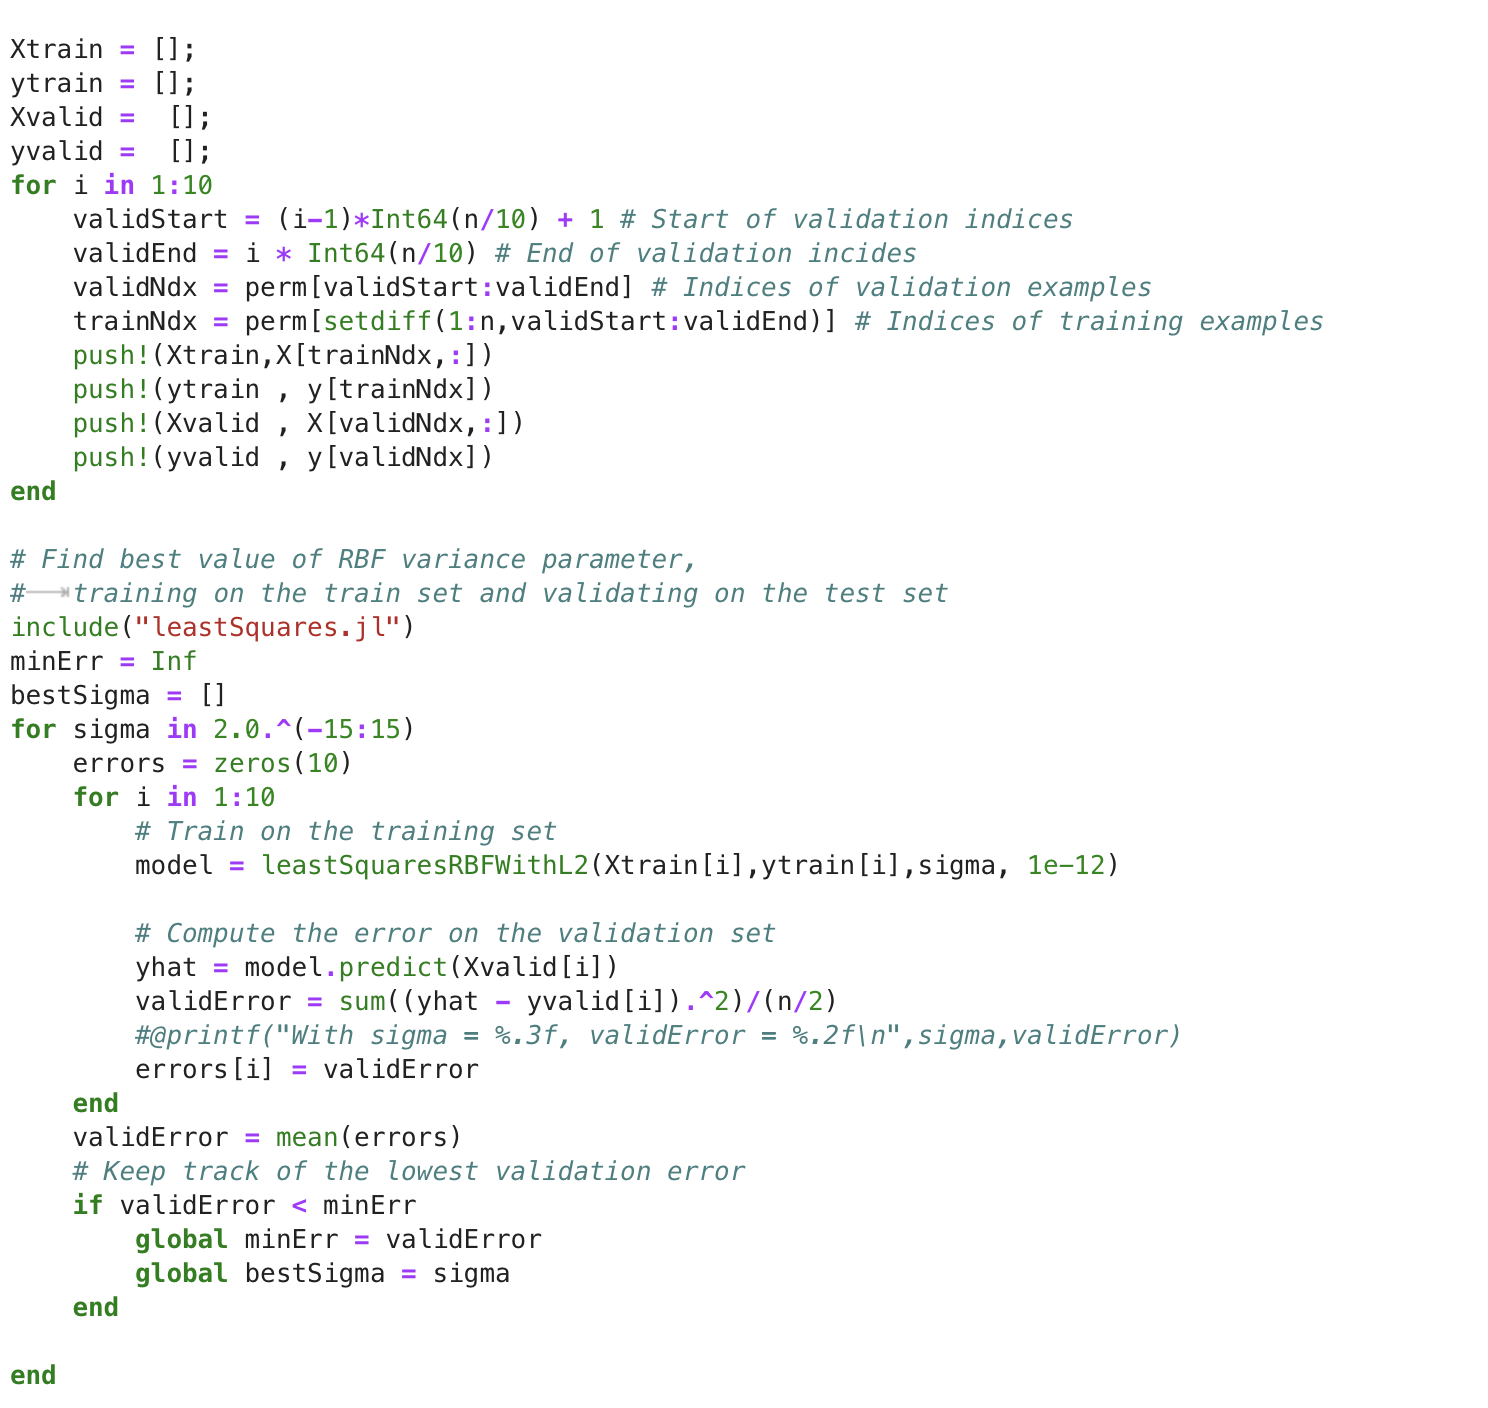
\includegraphics[width=10cm]{q12Code.png} The algurithm will now always choose 1 as $\sigma$ after run the code several times.}

\subsection{Cost of Non-Parametric Bases}

When dealing with larger datasets, an important issue is the dependence of the computational cost on the number of training examples $n$ and the number of features $d$. 
\blu{
\enum{
\item What is the cost in big-O notation of training a linear regression model with Gaussian RBFs on $n$ training examples with $d$ features (for fixed $\sigma$ and $\lambda$)?  \ans{$O(n^2d)$}
\item What is the cost of classifying $t$ new examples with this model? \ans{$O(ndt)$}
\item When is it cheaper to train using Gaussian RBFs than using the original linear basis? \ans{When feature is nore than number of examples.}
\item When is it cheaper to predict using Gaussian RBFs than using the original linear basis? \ans{Never}
}}


\section{Logistic Regression with Sparse Regularization}

If you run the function \emph{example\_logistic.jl}, it will:
\enum{
\item Load a binary classification dataset containing a training and a validation set.
\item ``Standardize'' the columns of $X$ and add a bias variable.
\item Apply the same transformation to $Xvalidate$.
\item Fit a least squares model, using the sign of $w^Tx_i$ to make predictions.
\item Report the number of features selected by the model (number of non-zero regression weights).
\item Report the error on the training and validation sets.
}
Least squares does ok as a binary classifier on this dataset, but it uses all the features (even though only the prime-numbered features are relevant) and the validation error is above the minimum achievable for this model (which is 1 percent, if you have enough data and know which features are relevant). In this question, you will modify this demo to use the logistic loss and to use different forms of regularization to improve on these aspects.


\subsection{Logistic Regression}

Instead of least squares, modify the script to use logistic regression. You can use the \emph{logReg.jl} file, which implements the training and prediction function for a logistic regresion classifier (using a  version of the \emph{findMin} function that does derivative checking for you and that uses more-clever choices of step-sizes). When you switch to using logistic regression, \blu{report how the following quantities change: the training error, validation error, and number of features}.
\ans{
    The training error goes to 0; and validation error is 0.082 lower than before. but number of none zeros remains unchanged.
}
\subsection{L2-Regularization}

Make a new function, \emph{logRegL2}, that takes an input parameter $\lambda$ and fits a logistic regression model with L2-regularization. Specifically, while \emph{logReg} computes $w$ by minimizing
\[
f(w) = \sum_{i=1}^n \log(1+\exp(-y_iw^Tx_i)),
\]
your new function \emph{logRegL2} should compute $w$ by minimizing
\[
f(w) = \sum_{i=1}^n \left[\log(1+\exp(-y_iw^Tx_i))\right] + \frac{\lambda}{2}\norm{w}^2.
\]
\blu{Hand in the objective function that your updated code minimizes, and using $\lambda=1.0$ report how the following quantities change: the training error, the validation error, the number of features used, and the number of gradient descent iterations.}
\ans{
    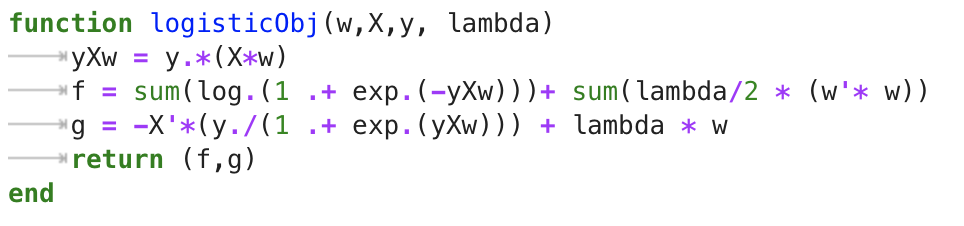
\includegraphics[width = 10cm]{Q22.png}
    numberOfNonZero = 101
trainError = 0.002
validError = 0.074
The training Error goes up but the validation error goes down, and Nomber of non zero stays the same.
}



\subsection{L1-Regularization}

Make a new function, \emph{logRegL1}, that takes an input parameter $\lambda$ and fits a logistic regression model with L1-regularization,
\[
f(w) = \sum_{i=1}^n \left[\log(1+\exp(-y_iw^Tx_i))\right] + \lambda\norm{w}_1.
\]
\blu{Hand in your \emph{logRegL1} code. Using this new code and $\lambda=1$, report the following quantities: the training error, the validation error, and the number of features the model uses.}


You should use the function \emph{findMinL1}, which implements a proximal-gradient method to minimize the sum of a differentiable function $g$ and $\lambda\norm{w}_1$,
\[
f(w) = g(w) + \lambda \norm{w}_1.
\]
 This function has a similar interface to \emph{findMin}, except that you (a) only provide the code to compute the function/gradient of the differentiable part $g$ and (b) need to provide the value $\lambda$. 

 \ans{ 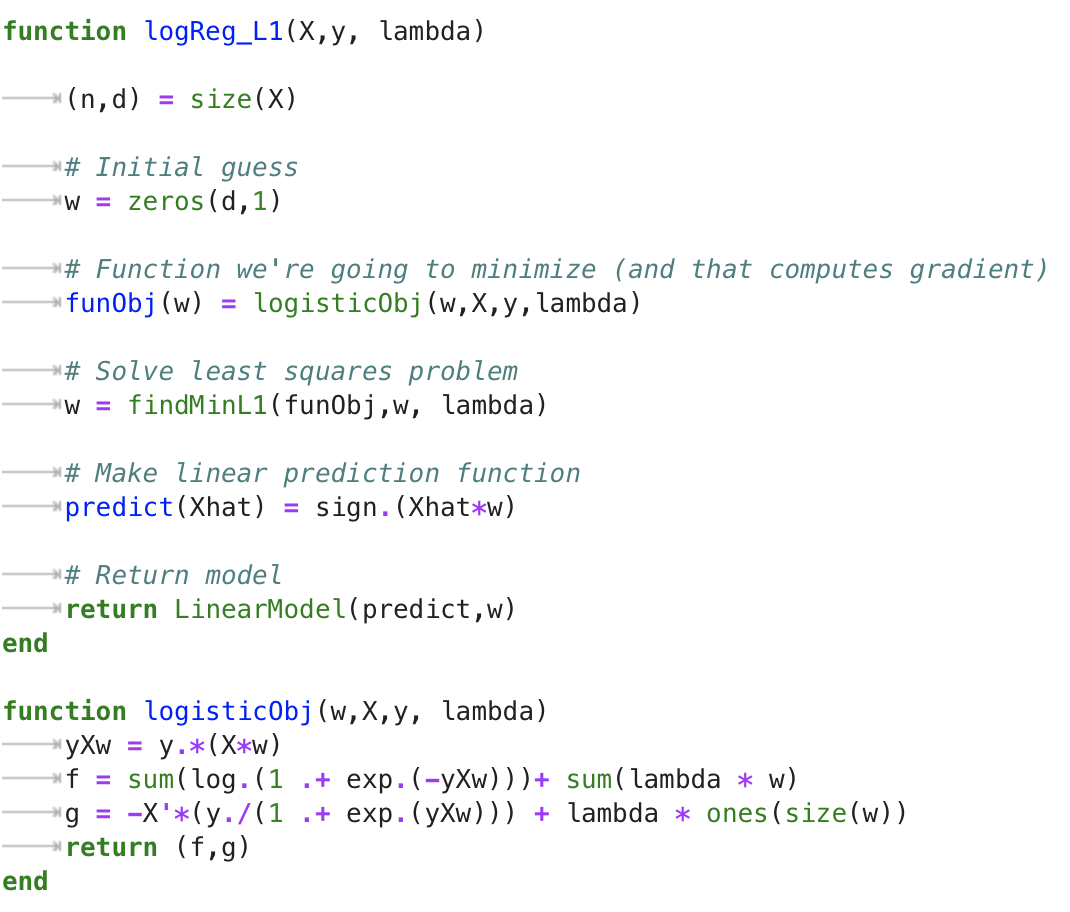
\includegraphics[width=10cm]{Q23.png}
     numberOfNonZero = 72
 trainError = 0.0
 validError = 0.048
 The number of feature used is smaller. The test error and validation error also goes down.
 }


\subsection{L0-Regularization}

The function \emph{logRegL0} contains part of the code needed to implement the \emph{forward selection} algorithm, which approximates the solution with L0-regularization,
\[
f(w) =  \sum_{i=1}^n \left[\log(1+\exp(-y_iw^Tx_i))\right] + \lambda\norm{w}_0.
\]
The `for' loop in this function is missing the part where we fit the model using the subset \emph{Sj}, then compute the score and updates the \emph{minScore/minS}. Modify the `for' loop in this code so that it fits the model using only the features \emph{Sj}, computes the score above using these features, and updates the \emph{minScore/minS} variables (if you want to turn off the diagonistics generated by \emph{findMin}, you can use \emph{verbose = false}).\footnote{Note that Julia doesn't like when you re-define functions, but if you change the variable \emph{Xs} it will actually change the behaviour of the \emph{funObj} that is already defined.}
\blu{Hand in your updated code. Using this new code, set $\lambda = 1$ and report: the training error, the validation error, and the number of features used.}

Note that the code differs a bit from what we discussed in class, since we assume that the first feature is the bias variable and assume that the bias variable is always included. Also, note that for this particular case using the L0-norm with $\lambda=1$ is equivalent to what is known as the Akaike information criterion (BIC) for variable selection.

\ans{
    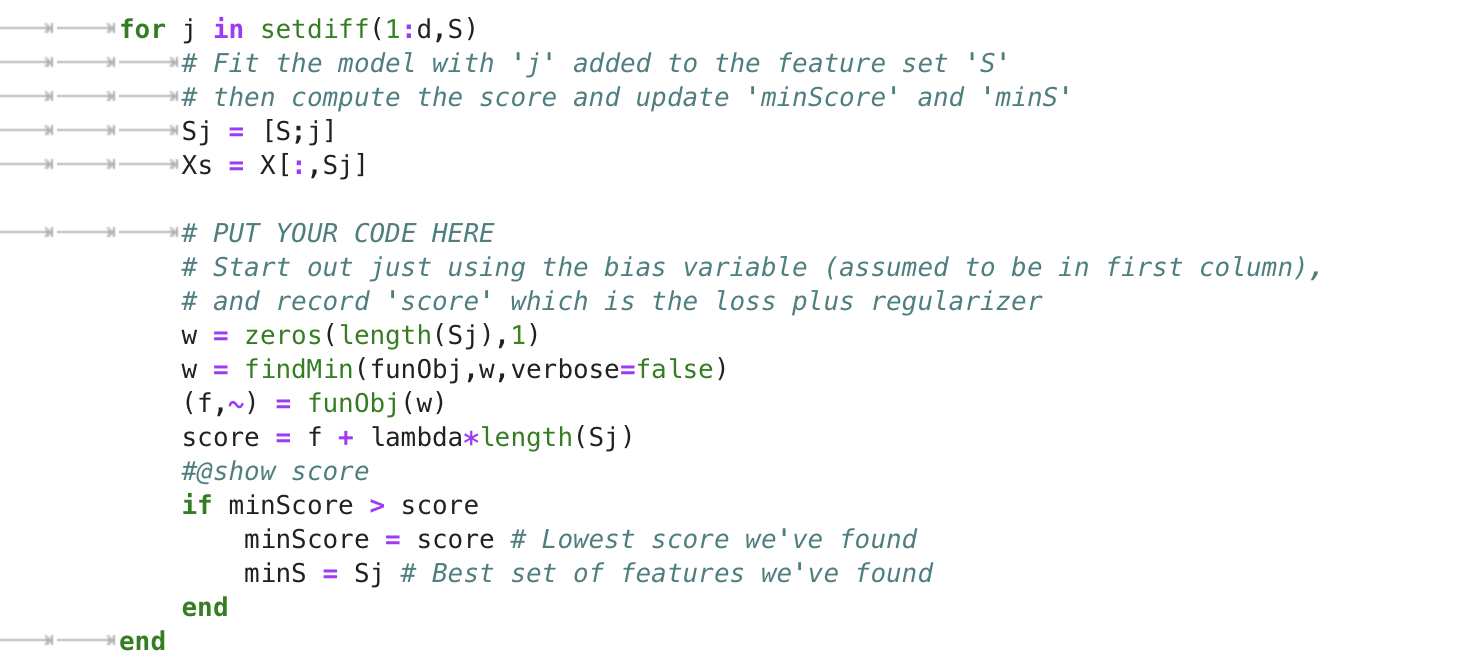
\includegraphics[width=10cm]{Q24.png}
    numberOfNonZero = 24
trainError = 0.0
validError = 0.018
The validation error goes down a lot, and number of features used is 24. They are all relevent. (1 2 3 5 7 11 13 17 19 23 31 37 41 43 47 53 59 67 71 73 79 83 89 101)
}


\section{Multi-Class Logistic}

The function \emph{example\_multiClass} loads a multi-class classification datasetwith $y_i \in \{1,2,3,4,5\}$ and fits a `one-vs-all' classification model using binary logistic regression, then reports the validation error and shows a plot of the data/classifier. The performance on the validation set is ok, but could be much better. For example, this classifier never  predicts that examples will be in class 1 (the green class).

\subsection{Softmax Classification}

Linear classifiers make their decisions by finding the class label $c$ maximizing the quantity $w_c^Tx_i$, so we want to train the model to make $w_{y_i}^Tx_i$ larger than $w_{c'}^Tx_i$ for all the classes $c'$ that are not the true label $y_i$. 
Here, $c$ is a possible label and $w_{c'}$ is \red{row} $c'$ of $W$. Similarly, $y_i$ is the training label, $w_{y_i}$ is \red{row} $y_i$ of $W$, and in this setting we are assuming a discrete label $y_i \in \{1,2,\dots,k\}$. Before we move on to implementing the softmax classifier to fix the issues raised in the introduction, let's do a simple example:

Consider the dataset below, which has $10$ training examples, $2$ features, and $3$ class labels:
\[
X = \begin{bmatrix}0 & 1\\1 & 0\\ 1 & 0\\ 1 & 1\\ 1 & 1\\ 0 & 0\\  1 & 0\\  1 & 0\\  1 & 1\\  1 &0\end{bmatrix}, \quad y = \begin{bmatrix}1\\1\\1\\2\\2\\2\\3\\3\\3\\3\end{bmatrix}.
\]
Suppose that you want to classify the following test example:
\[
\hat{x} = \begin{bmatrix}1 \\ 1\end{bmatrix}.
\]
Suppose we fit a multi-class linear classifier using the softmax loss, and we obtain the following weight matrix:
\[
W = 
\red{\begin{bmatrix}
+2 & -1\\
+2 & +2\\
+3 & -1\\
\end{bmatrix}}
\]
\blu{
\enum{
\item Why are the weights of this model a \red{$3 \times 2$} matrix? \ans{Because there are 3 kinds of labels in the training set. And there are 2 freatures for one example.}
\item Under this model, what class label would we assign to the test example? (Show your work.) \ans{$Wx= \begin{bmatrix}
    +2 + -1\\
    +2 + +2\\
    +3 + -1\\
    \end{bmatrix} = \begin{bmatrix}
        1\\
        4\\
        2\\
        \end{bmatrix}$ \\
        So it will presict 2 as it has the largest value. }
}}





\subsection{Softmax Loss}

Using a one-vs-all classifier hurts performance because the classifiers are fit independently, so there is no attempt to calibrate the columns of the matrix $W$. An alternative to this independent model is to use the softmax loss probability,
\[
p(y_i \cond W, x_i) = \frac{\exp(w_{y_i}^Tx_i)}{\sum_{c=1}^k\exp(w_c^Tx_i)}.
\]
The loss function corresponding to the negative logarithm of the softmax probability for $n$ training examples is given by
\[
f(W) = \sum_{i=1}^n \left[-w_{y_i}^Tx_i + \log\left(\sum_{c' = 1}^k \exp(w_{c'}^Tx_i)\right)\right].
\]
\blu{Derive the partial derivative of this loss function with respect to a particular element $\red{W_{cj}}$}. Try to simplify the derivative as much as possible (but you can express the result in summation notation).
\ans{The diravitive respect to $w_{cj}$ is $\sum _{i=1}^n [-X_{ij}*I(y_1=c) + (w_{cj}x_{ij})]$}

Hint: for the gradient you can use $x_{ij}$ to refer to element $j$ of example $i$. For the first term you can use an `indicator' function, $I(y_i = c)$, which is $1$ when $y_i = c$ and is $0$ otherwise. Note that you can use the definition of the softmax probability to simplify the derivative.



\subsection{Softmax Classifier}

Make a new function, \emph{softmaxClassifier}, which fits $W$ using the softmax loss from the previous section  instead of fitting $k$ independent classifiers. \blu{Hand in the code and report the validation error}.

Hint: you will want to use the \emph{derivativeCheck} option in \emph{findMin.jl} to check that your gradient code is correct. Also, note that \emph{findMin.jl} expects that the parameter vector and gradient are \emph{column vectors}. The easiest way to work around these issues is to use the \emph{reshape} command: call \emph{findMin.jl} with a $dk \times 1$ vector $w$ and at the start of your objective function reshape $w$ to be a $d \times k$ matrix $W$, then compute the $d \times k$ matrix of partial derivatives and finally reshape this to be the $dk \times 1$ gradient vector.

\subsection{Cost of Multinomial Logistic Regression}

Assuming that we have
\items{
\item $n$ training examples.
\item $d$ features.
\item $k$ classes.
\item $t$ testing examples.
\item $T$ iterations of gradient descent for training.
}
\blu{\enum{
\item In $O()$ notation, what is the cost of training the softmax classifier?
}}



\section{Very-Short Answer Questions}

\enum{
\item Consider performing feature selection by measuring the ``mutual information'' between each column of $X$ and the target label $y$, and selecting the features whose mutual information is above a certain threshold (meaning that the features provides a sufficient number of ``bits'' that help in predicting the label values). Without delving into any details about mutual information, what is a potential problem with this approach?
\item Why do we use forward selection instead of exhaustively search all subsets in search and score methods?
\item What is a setting where you would use the L1-loss, and what is a setting where you would use L1-regularization?
\item Among L0-regularization, L1-regularization, and L2-regularization: which yield convex objectives? Which yield unique solutions? Which yield sparse solutions?
\item What is the effect of $\lambda$ in L1-regularization on the sparsity level of the solution? What is the effect of $\lambda$ on the two parts of the fundamental trade-off?
\item Suppose you have a feature selection method that tends not generate false positives but has many false negatives (it misses relevant variables). Describe an ensemble method for feature selection that could improve the performance of this method.
\item How does the hyper-parameter $\sigma$ affect the shape of the Gaussian RBFs bumps? How does it affect the fundamental tradeoff?
\item What is the main problem with using least squares to fit a linear model for binary classification?
\item Suppose a binary classification dataset has 3 features. If this dataset is ``linearly separable'', what does this precisely mean in three-dimensional space?
\item When searching for a good $w$ for a linear classifier, why do we use the logistic loss instead of just minimizing the number of classification errors?
\item For a linearly-separable binary classification problem, how does an SVM classifier differ from a classifier found using the perceptron algorithm?
\item Which of the following methods produce linear classifiers? (a) binary least squares as in Question 3, (b) the perceptron algorithm, (c) SVMs, (d) logistic regression, and (e) KNN with $k=1$ and $n=2$.
\item Why do we use the polynomial kernel to implement the polynomial basis when $d$ and $p$ (degree of polynomial) are large?
\item Suppose we want to fit a multi-class logistic regression model, but the class labels do not form convex regions. How could we modify multi-class logistic regression to fit non-convex regions?
}



\end{document}